\expandafter\newcommand\csname dataXGBvifcap1metrictab\endcsname{
\begin{table}[H]
\begin{tabular}
{| 
 p{\dimexpr0.2\textwidth-2\tabcolsep-\arrayrulewidth\relax}| 
 p{\dimexpr0.2\textwidth-2\tabcolsep-\arrayrulewidth\relax}| 
 p{\dimexpr0.2\textwidth-2\tabcolsep-\arrayrulewidth\relax}| 
 p{\dimexpr0.2\textwidth-2\tabcolsep-\arrayrulewidth\relax}| 
 p{\dimexpr0.2\textwidth-2\tabcolsep-\arrayrulewidth\relax}| 
}\hline 
\textbf{} &\textbf{f1-score} &\textbf{precision} &\textbf{recall} &\textbf{support} \\ \hline 
CANDIDATE &0.649 &0.725 &0.588 &170.0 \\ \hline 
CONFIRMED &0.862 &0.823 &0.905 &241.0 \\ \hline 
FALSE POSITIVE &0.939 &0.93 &0.949 &391.0 \\ \hline 
accuracy &0.859 &0.859 &0.859 &0.859 \\ \hline 
macro avg &0.817 &0.826 &0.814 &802.0 \\ \hline 
weighted avg &0.854 &0.854 &0.859 &802.0 \\ \hline 
\end{tabular} 
\end{table}
}
\begin{figure}[H]
                \centering
                \begin{subfigure}{.49\textwidth}
                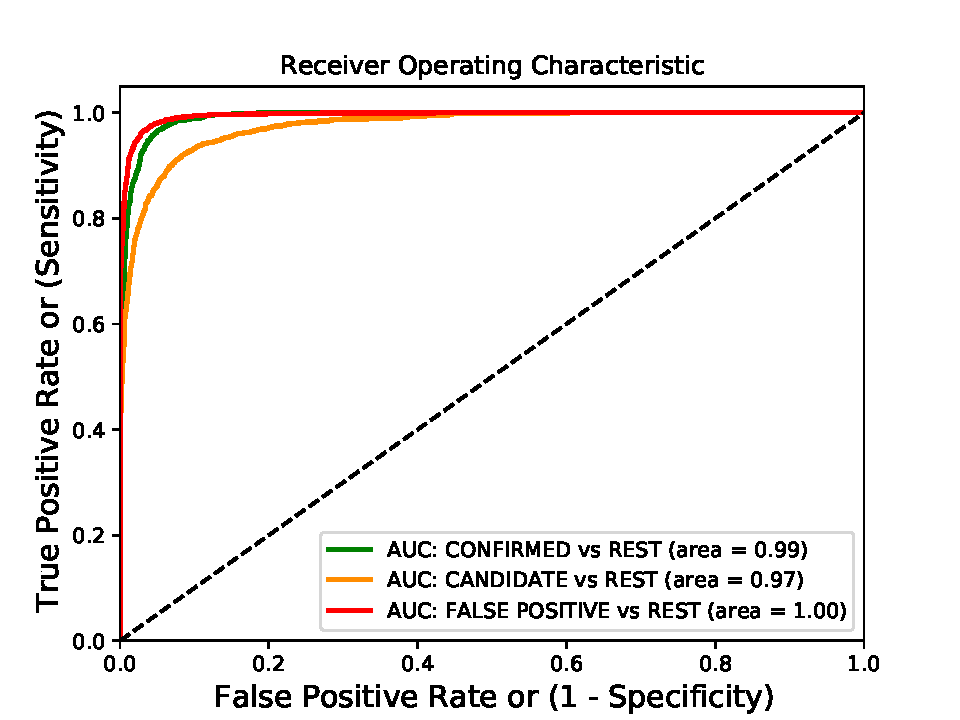
\includegraphics[width = 1\textwidth]{data/XGB_vif_cap1_overfit_roc.pdf}
                \end{subfigure}
                \begin{subfigure}{.49\textwidth}
                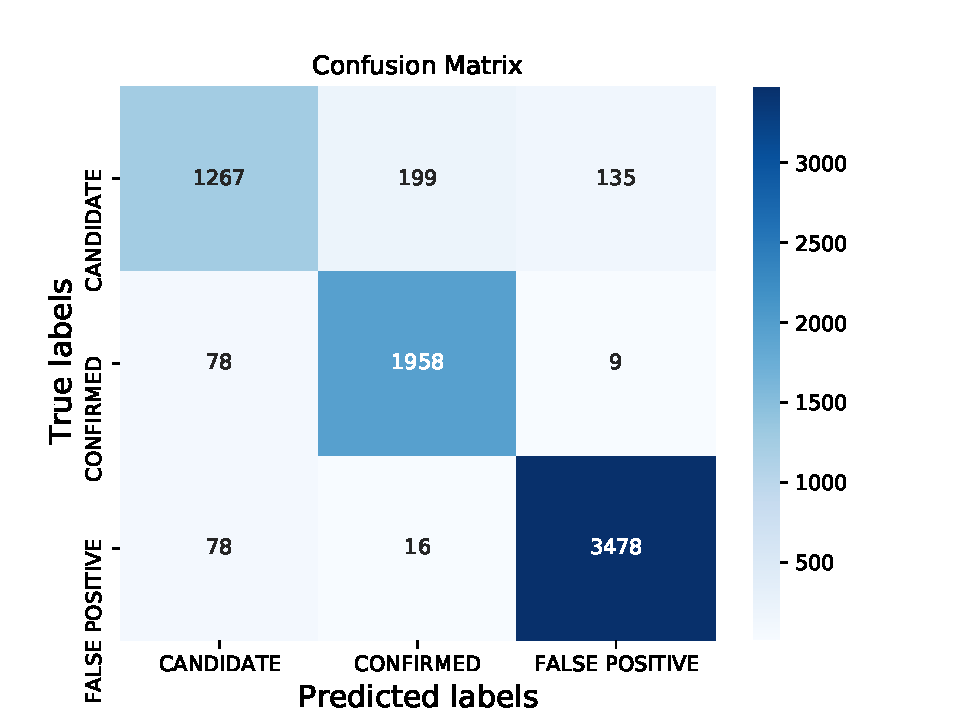
\includegraphics[width = 1\textwidth]{data/XGB_vif_cap1_overfit_cm.pdf}
                \end{subfigure}
                \begin{subfigure}{.49\textwidth}
                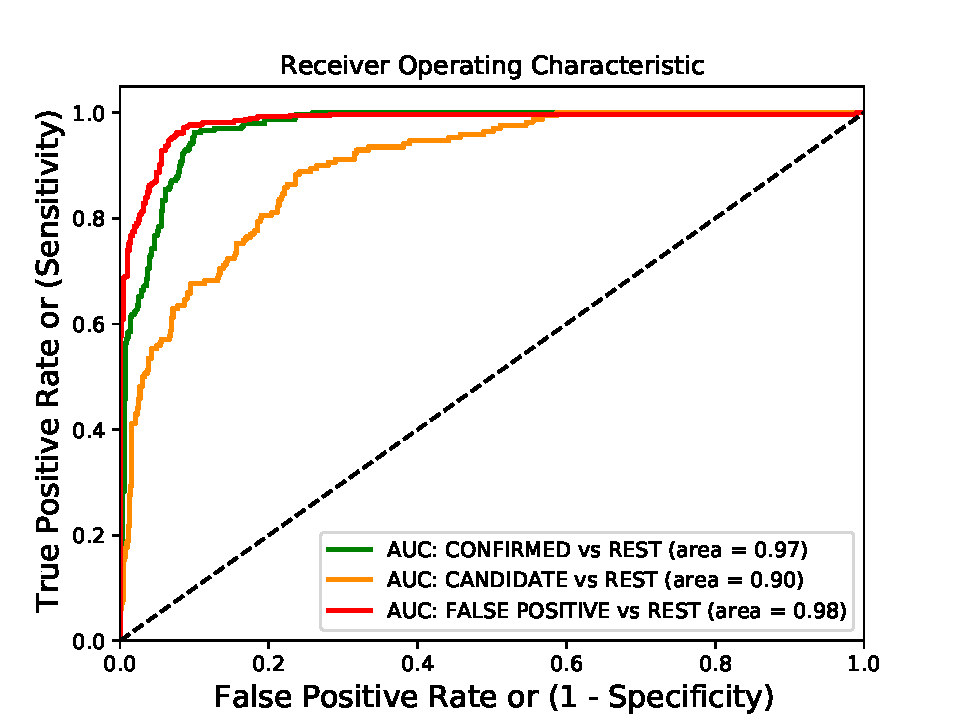
\includegraphics[width = 1\textwidth]{data/XGB_vif_cap1_roc.pdf}
                \end{subfigure}
                \begin{subfigure}{.49\textwidth}
                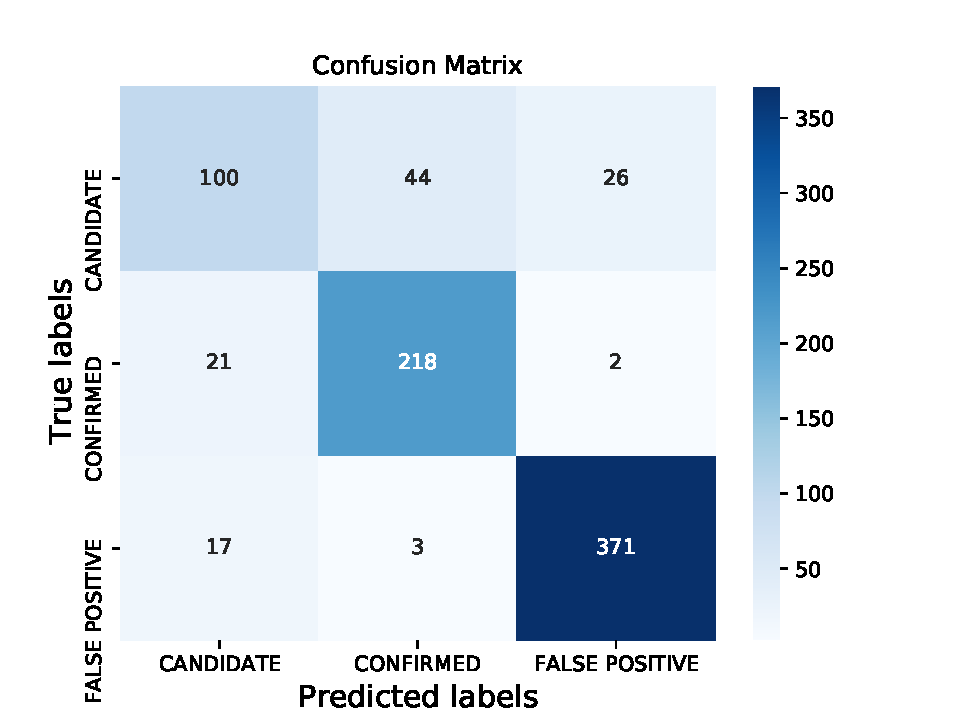
\includegraphics[width = 1\textwidth]{data/XGB_vif_cap1_cm.pdf}
                \end{subfigure}
                \begin{subfigure}{1\textwidth}
                \csname dataXGBvifcap1metrictab\endcsname
                \end{subfigure}
                \caption{XGBvifcap1: Top Row: overfit test. Middle and bottom row test data}
                \label{fig:data/XGB_vif_cap1_roc}
                \end{figure}